\documentclass[french]{report}
\usepackage[utf8]{inputenc}
\usepackage[a4paper,total={5.8in, 9in}]{geometry}
\usepackage[T1]{fontenc}
\usepackage{babel}
\usepackage[autolanguage]{numprint}
\usepackage{hyphenat}
\usepackage{gensymb}
\usepackage{graphicx}
\usepackage{titlesec}
\usepackage{minted}
\usepackage{listings}
\usepackage{enumitem}
\usepackage{xcolor}
\usepackage{pythonhighlight}
\definecolor{blue}{RGB}{51,131,255}
\newcommand\tab[1][1cm]{\hspace*{#1}}
\usepackage[skins]{tcolorbox}
\graphicspath{{img/}}

\title{Lockatme\\A screen lock with facial recognition abilities\\Final report}
\date{\today}
\author{David Anandanadaradja, Sagar Gueye, Bruno Inec,\\ Matthieu Kirschleger,
Pierre-Louis Sergent}

\begin{document}
    \maketitle

    \tableofcontents

\chapter{Antériorité}
\newpage

\section{Présentation des membres du groupe}

\subsection{Contexte}
Dans le cadre de notre DUT Informatique à l’IUT Lyon 1, nous sommes tenus de
réaliser un projet tuteuré durant le second semestre. Ce projet s’étendant
également sur le troisième semestre, il a pour but de répondre à une
problématique précise et de mettre en oeuvre les compétences acquises au cours
de la formation. Il a aussi vocation à faire découvrir de nouveaux domaines et
il nous permettra d’élargir nos savoirs à travers une auto-formation.

\vspace{0.5cm}
Ce projet se découpe en deux axes :
\begin{itemize}[label=\textbullet, font=\normalfont \color{blue}]
  \item{Rédaction du cahier des charges (second semestre)}
  \item{Réalisation du projet en lui même (troisième semestre)}
\end{itemize}
\vspace{0.5cm}

Malgré une liste de sujets proposés, notre groupe a voulu suivre ses propres
motivations (présentées plus loin dans ce document) et a choisi de proposer un
sujet à M. Vidal. L’intitulé est le suivant : Verrouillage et déverrouillage
d’écran par reconnaissance faciale sous Linux.

\subsection{Organisation et membres}
L’équipe chargée de ce projet est constituée
\begin{itemize}[label=\textbullet, font=\normalfont \color{blue}]
  \item{Tuteur du projet : M. Vincent VIDAL}
  \item{Chef du projet : M. Bruno INEC}
  \item{Membres : M. David ANANDANADARADJA, Mme Sagar GUEYE, M. Matthieu
        KIRSCHLEGER et M. Pierre-Louis SERGENT}
\end{itemize}

\subsection{Compétences}
Notre projet comporte deux contraintes principales : il nécessite une bonne
connaissance du langage Python et une
maîtrise de Linux. L’impulsion de ces choix vient en grande partie du chef de
projet qui possède une expérience importante dans ces deux domaines. David et
Pierre-Louis possèdent quant à eux une expérience modérée dans l’utilisation de
Linux (distribution Arch). L’ensemble des compétences individuelles est résumé
ci-après :
\\

\textbf{Python} :
\begin{itemize}[label=\textbullet, font=\normalfont \color{blue}]
  \item{Confirmé : Bruno INEC}
  \item{Intermédiaire : Pierre-Louis SERGENT}
  \item{Débutant : Sagar GUEYE, Matthieu KIRSCHLEGER, David ANANDA}
\end{itemize}

\textbf{Linux} :
\begin{itemize}[label=\textbullet, font=\normalfont \color{blue}]
  \item{Confirmé : Bruno INEC}
  \item{Intermédiaire : David ANANDA, Pierre-Louis SERGENT}
  \item{Débutant : Sagar GUEYE, Matthieu KIRSCHLEGER}
\end{itemize}

\vspace{0.5cm}

Comme le montre le listing précédent, les compétences du groupe sont très
disparates. Cela peut apparaître comme une contrainte, mais en réalité cela
constitue une véritable opportunité pour tous les membres. Ils vont ainsi
pouvoir se former dans les domaines ci-après. Ils sont essentiels pour la
suite des études et pour le milieu professionnel.
\newpage
\vspace{0.5cm}
\begin{itemize}[label=\textbullet, font=\normalfont \color{blue}]
  \item{Programmation : Linux, Python}
  \item{Rédaction cahier des charges : \LaTeX}
  \item{Travail en équipe : réunion, communication, CI, modèle de
  développement}
\end{itemize}
\vspace{0.5cm}

Nous étions donc motivés pour nous lancer dans un sujet avec nombre d’inconnus
mais qui allait être fort enrichissant.


\section{Présentation du projet}

\subsection{Buts}
Le but premier de l’application est de déverrouiller un écran d’ordinateur, à
l’aide d’une caméra, par reconnaissance faciale. Cependant cela implique de
mettre en place un verrouillage d’écran sous Linux. Les URS spécifiques seront
décrit plus tard dans ce document.

\subsection{Motivations}
Trois membres du groupe utilisent Arch Linux qui est une distribution minimale
de Linux. Le fait de quitter Windows leur a permis de pleinement se concentrer
sur la machine à un plus bas niveau, avec tous les avantages de liberté
qu’offre une plateforme open source, mais aussi toutes les contraintes qui sont
très formatrices et qui forcent à se pencher d’avantage sur le fonctionnement
de ce système d’exploitation. Les trois utilisateurs cherchaient une manière de
verrouiller/déverrouiller leur écran de manière sécurisée. Et l’idée de ce
projet a fleuri suite à un article présent dans le magazine Linux
Magazine/France n{\degree}203 : “Mettez en place un système de reconnaissance faciale”.

\subsection{Linux}
Le développement du logiciel se fera sur Linux. Un tel projet
sur Windows aurait été bien plus difficile concernant l’implémentation système
mais aussi le code de l’application. De plus, l’OS est largement privilégié par
les développeurs dans le monde de la programmation. C’est pourquoi nous avons
choisi de réaliser notre projet sous Linux, qui s’adressera donc à un public
famillié avec la CLI (Command Line Interface) et les autres aspects techniques.
Des interfaces seront potentiellement développées à terme pour les utilisateurs
de distributions plus user-friendly (comme Ubuntu).

\subsection{Open Source}
Le développement du projet se fera de manière complètement transparente et donc
en open source. Ce choix est assez logique lorsque l’on réalise un programme
pour Linux, car il s’inscrit exactement dans la politique des développeurs qui
ont réalisé ce dernier. Cela possède de nombreux avantages : possibilité pour
la communauté de contribuer au projet au travers de modifications du code,
commentaires, rapport de bug, \ldots

\chapter{Gestion de projet}

\newpage

\section{Stratégie de développement}

\subsection{Méthodologie voulue}
Lors de la réalisation du cahier des charges, nous avions réfléchi à la mise en
place d'une méthodologie agile: SCRUM, afin de conserver une bonne visibilité sur le
projet. Ainsi, nous souhaitions réaliser des cycles; un cycle correspondant au
lapse de temps entre deux réunions avec le tuteur; pour que ce dernier soit au
maximum impliqué dans le projet et qu'il puisse nous aiguiller en cas de problème.
\\
\\
La méthodologie SCRUM implique également une intégration continue pour faire
paraître à la fin de chaque cycle une nouvelle version. Pour cela l'idée était
d'utiliser un service de décentralisation basé sur Git (GitHub), pour pouvoir merged les
différentes branches sur la branche master.

\subsection{Application réelle au projet}
La réalisation du projet en lui même a nécessité de longues heures de recherches
individuelles (\emph{cf. 2.2.2 Liste des tâches}), notamment pour lire de la documentation et faire des "boûts" de
code afin de mieux cerner ce que nous allions faire. C'est pourquoi la phase de développement à
été plus courte que prévu.
\\
\\
Malgré cela, nous avons réalisé de manière régulière des \emph{stand-ups} pour
répartir les recherches et pour parler de nos avancements et de nos problèmes.
Lorsque nous avions
plus de temps (période de vacances), il nous arrivait aussi de travailler
quotidiennement en open-space en équipe de 2-3 personnes pour permettre un
retour plus rapide sur le travail effectué et une mise en commun.
\\
\\
Pour ce qui est de la méthode SCRUM, nous avons mis en place des sprints de une
à deux semaines. À la fin de ces derniers nous nous retrouvions, à
l'occasion des stand-ups, afin de fermer les tickets résolus et d’ouvrir de
nouveaux tickets pour le sprint d’après. Les outils qui nous ont servi
pour exploiter le potentiel de cette méthodologie
sont \emph{Taiga} pour le suivi et la gestion des tickets (\emph{cf. Annexe ~\ref{fig:Taiga}})
et \emph{Discord} pour la communication par message ou vidéo.
\\
\\
L'intégration continue a aussi été mise en place. Nous avons bien
utilisé GitHub pour la mise en commun du travail. Chacun travaillant sur sa
branche. Cependant, malgré beaucoup de recherche, il résultait assez peu de code. Il
était donc difficile de séparer les tâches sur plusieurs branches pour ensuite
merge sur master. La plupart du temps c'etait donc le chef du projet qui
implémentait les features, en se basant sur les recherches de tout le monde (sans
pour autant tout faire \emph{cf. 2.2.2 Liste des tâches}).

\section{Phases du projet – distribution des tâches}

\subsection{Rétrospective - diagramme de Gantt specification}
Voir ci dessous le diagramme de Gantt que nous avions réalisé lors du cahier
des charges pour le S2.

\begin{figure}[h]\label{fig:gantt}
  \includegraphics[width=\linewidth]{Gantt}
  \caption{diagramme de Gantt}
  \label{fig:gantt}
\end{figure}

Etant donné que le sujet était très complexe et comportait de nombreuses zones
d'ombres, nous avions fait un diagramme de Gantt, approximatif, quant à la durée
des différentes tâches, ainsi qu'à leurs enchaînements. Nous allons voir dans
la partie qui suit, que ce diagramme n'a pas été respecté. Des tâches ont été
largement sous-estimées, notamment à cause de l'aspect technique de certains
éléments qui ont été bloquant. Certaines tâches ont été supprimées ou requalifiées.
Suite à nos recherches nous avons changé de stratégie de développement plusieurs
fois, il y a donc eu un changement dans les technologies utilisées ainsi que dans les
moyens pour arriver à nos fins.
\\
Il existe cependant une certaine ressemblance, concernant les grandes parties,
entre l'ancien diagramme et le déroulement réel. A savoir :

\vspace{0.5cm}
\begin{itemize}[label=\textbullet, font=\normalfont \color{blue}]
  \item{\textbf{Recherche sur l'algorithme pour la reconnaissance faciale}}
  \item{\textbf{Verrouillage et déverrouillage de l'écran, implémentation système}}
  \item{\textbf{Upload pip, amélioration, test}}
\end{itemize}
\vspace{0.5cm}

\subsection{Répartition réalisée}

\subsubsection{Difficultés rencontrées}
Comme dit auparavant, de nombreuses difficultés ont été rencontrées plus tôt que prévu.
Voici une liste exhaustive de celles-ci :

\vspace{0.5cm}
\begin{itemize}[label=\textbullet, font=\normalfont \color{blue}]
  \item{\textbf{Répartition des recherches}}\\
Le sujet abordé était très technique et précis, il nécessitait donc beaucoup de
recherches. Mais la répartition était plutôt compliquée étant donné que, idéalement,
il aurait fallu que tout le monde possède une connaissance globale des technologies,
qui pouvait théoriquement nous servir pour le développement.\\

  \item{\textbf{Exploitation des recherches, mise en commun}}\\
Par la suite, les nombreuses heures de recherches(\emph{cf. 2.2.2 Liste des tâches}) ne nous avançaient guère pour la
réalisation de notre projet. Il était difficile d'avoir une vision sur le long
terme, quand nous stagnions, parfois plusieurs jours, sur un aspect compliqué. Il
n'était pas évident de savoir concrètement à quoi allait nous servir certaines
connaissances (beaucoup n'ont finalement pas été utile). La mise
en commun prenant beaucoup de temps. Il était parfois nécessaire de rédiger un
petit document pour résumer les choses apprises durant une semaine afin de mieux
pouvoir les exploiter et de déterminer si oui ou non elles seront utiles.\\

  \item{\textbf{Compréhension, avancement éparse}}\\
Et donc suite à cela, venait le temps de la compréhension. Certains aspects techniques
liés à l'architecture linux bloquaient certains. L'évolution des connaissances de
chacun était assez éparpillé. De plus en plus, chacun recherchait de son propre
côté en fonction de ses avancements. Cela à mener à une dispersion, néfaste pour
l'intérêt commun du groupe.\\

  \item{\textbf{Changement fréquent de stratégie suite à de nouvelles découvertes}}\\
Nos avancements nous ont irrémédiablement mené à changer d'idée plusieurs fois
pour le développement (\emph{cf. 2.2.2 Chronologie}). Il était donc assez
frustrant de se rendre compte que des heures de travail ne seront peut être pas
utilisés concrètement dans le rendu final. Mais cela fait partie du projet,
c'est à dire que pour en arriver au meilleur résultat possible, il était important
d'explorer toutes les pistes possibles pour découvrir de nouvelles choses et ainsi
réaliser le code le plus pertinent possible, dans le cadre de la philosophie de lockatme.\\

  \item{\textbf{Impliquation de tout le groupe}}\\
Evidemment vu la liste qui est en train d'être faite, il est assez simple de deviner
que cette phase a été bien compliqué pour certains membres du groupe, qui ont pu
prendre du retard dans la compréhension de l'avancement. Mais il était quand même
important de tenir tout le monde informé, notamment à travers des réunions régulières.
La part de développement de chacun était inégale, mais il était essentiel que
tout le monde apporte sa contribution au projet. Les personnes moins à l'aise
compensaient avec des tâches liées à la gestion du projet. De plus, il est essentiel que chaque membre ait
connaissance des aspects techniques de l'application.\\

  \item{\textbf{Répartition des tâches lors du développement}}\\
En lien avec le point précédent et avec un paragraphe du 2.2, dans le développement
final il y avait assez peu de code (même si très complexe \emph{cf. 3.2}). Il n'y avait pas de
séparation possible avec differentes couches, comme peu nous offrir le modèle MVC
par exemple. C'est donc essentiellement le chef de groupe qui a implémenté la partie
finale(\emph{cf. 2.2.2 Liste des tâches}). Cela ne veut pas dire qu'il a fait tout
le travail étant donné que les recherches de chacuns ont été prises en compte. Il
faut garder à l'esprit que dans ce projet la partie de reflexion et de recherche
représente 80\% du temps de travail.\\

\end{itemize}

\subsubsection{Chronologie}

\vspace{0.5cm}
\textbf{Quelles recherches?}\\

  L’idée de la reconnaissance faciale nous était venue d’un article de magazine,
  ainsi la documentation sur cette algorithme est très abondante avec de
  multiples solutions. Cependant la partie implémentation système et
  verrouillage sur X11 nous était complètement inconnue, il nous fallait donc
  nous plonger dans la recherche et la documentation pour ces deux aspects.
\\ \\
  La première question a été, comment le système gère-t’il le déverrouillage?
\\ \\
  L’ensemble du groupe s’est donc plongé dans cette recherche.

  \vspace{0.5cm}
\newpage
  \textbf{PAM: Pluggable Authentication Modules} \emph{(Bruno, David,
  Pierre-Louis, travail en parallèle de Python into C)}\\\\
En nous penchant sur des applications de lock sous Linux, telles que i3lock,
lightDM, nous nous sommes rendus compte qu’elles utilisent toute PAM.
Ce dernier permet au travers de configs files, contenant des modules, de
gérer l’authentification. Les applications font appel à PAM en passant en
paramètre le nom de la config file, qui elle même contient des modules
d’authentification.

  \begin{figure}[h]
    \begin{center}
    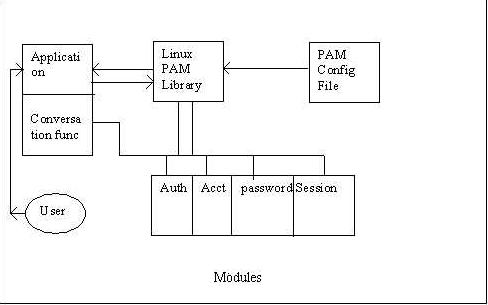
\includegraphics[width=0.8\linewidth]{pam}
    \caption{schéma explication PAM}
  \end{center}
  \end{figure}

  Nous nous sommes donc répartis les recherches à partir de là, en trois parties
  (issues de la documentation officielle):
  \vspace{0.5cm}
  \begin{itemize}[label=\textbullet, font=\normalfont \color{blue}]
    \item{\textbf{The System Administrators' Guide (Pierre-Louis)}}

    \vspace{0.05cm}

Cette partie concerne les PAM config file contenues dans le répertoire
\verb|/etc/pam.d|. Elles contiennent les modules PAM qui seront utilisés suite à
l’appel de PAM par l’application. Il s’agit d’une syntaxe particulière où les
modules sont regroupés en "type group" : account, auth, password et session.
Après les types groups, sur la même ligne, vient la "control value", qui va
définir le comportement de l’application en fonction des valeurs de retour des
modules. Par exemple: required, sufficient, include, optional… Après la control
value vient le nom du module PAM utilisé. Ensuite le quatrième argument
constitue des options diverses que nous ne détailleront pas ici, car inutile
pour notre projet.
\\ \\
    Exemple: system-auth \\

    auth      required  \texttt{pam\_unix.so}   \texttt{try\_first\_pass
    nullok} \\
    auth      optional  \texttt{pam\_permit.so} \\
    auth      required  \texttt{pam\_env.so} \\

    account   required  \texttt{pam\_unix.so} \\
    account   optional  \texttt{pam\_permit.so} \\
    account   required  \texttt{pam\_time.so} \\
\newpage
    password  required  \texttt{pam\_unix.so}   \texttt{try\_first\_pass nullok
    sha512 shadow} \\
    password  optional  \texttt{pam\_permit.so} \\

    session   required  \texttt{pam\_limits.so} \\
    session   required  \texttt{pam\_unix.so} \\
    session   optional  \texttt{pam\_permit.so} \\

\vspace{0.5cm}

    \item{\textbf{The Module Writers' Guide (Bruno)}}

    \vspace{0.05cm}

Sur l’exemple du dessus on voit que le troisième argument de chaque ligne est
un module PAM. Il est possible d’écrire soit même un module en C. C’est ce qui
est traité dans cette partie. Cependant cet aspect est très lourd à comprendre.
Nous nous sommes donc reposé sur des exemples tel que le repository simple-pam
trouvé sur github(https://github.com/beatgammit/simple-pam). On a donc pu comprendre que chaque type group peut être
gérer avec une fonction qui retourne \texttt{PAM\_SUCCESS ou PAM\_ERR}.
\\ \\
    Exemple:

  \begin{minted}{c}

#include <security/pam_appl.h>
#include <security/pam_modules.h>

/* expected hook, this is where custom stuff happens */
PAM_EXTERN int pam_sm_authenticate( pam_handle_t *pamh, int flags,int argc,
  const char **argv ) {
	int retval;

	const char* pUsername;
	retval = pam_get_user(pamh, &pUsername, "Username: ");

	if (retval != PAM_SUCCESS) {
		return retval;
	}

	if (strcmp(pUsername, "papalouis") != 0) {
		return PAM_AUTH_ERR;
	}

	return PAM_SUCCESS;
}
\end{minted}

\vspace{0.5cm}

    \item{\textbf{The Application Developers' Guide (David)}}

    \vspace{0.05cm}

  Cette partie concerne l’appel du module PAM au sein d’une application. Nous
  avons retenu que toute utilisation de PAM débute avec un \texttt{pam\_start()}
  qui contient la config file souhaité. Ensuite si l’appel s’est fait
  correctement, on peut utiliser la fonction \texttt{pam\_authenticate()} par
  exemple pour lancer le processus d’authentification par mot de passe ou
  autre, en fonction des modules utilisés. A la fin du programme il faut fermer
  le PAM en utilisant \texttt{pam\_end()}.
\\ \\
\newpage
    Exemple:

  \begin{minted}{c}

#include <security/pam_appl.h>
#include <security/pam_misc.h>
#include <stdio.h>

const struct pam_conv conv = {
	misc_conv,
	NULL
};

int main(int argc, char *argv[]) {
	pam_handle_t* pamh = NULL;
	int retval;
	const char* user = "nobody";

	if(argc != 2) {
		printf("Usage: app [username]\n");
		exit(1);
	}

	user = argv[1];

	retval = pam_start("face-auth-test", user, &conv, &pamh);

	// Are the credentials correct?
	if (retval == PAM_SUCCESS) {
		printf("Credentials accepted.\n");
		retval = pam_authenticate(pamh, 0);
	}

	// Can the accound be used at this time?
	if (retval == PAM_SUCCESS) {
		printf("Account is valid.\n");
		retval = pam_acct_mgmt(pamh, 0);
	}

	// Did everything work?
	if (retval == PAM_SUCCESS) {
		printf("Authenticated\n");
	} else {
		printf("Not Authenticated\n");
	}

	// close PAM (end session)
	if (pam_end(pamh, retval) != PAM_SUCCESS) {
		pamh = NULL;
		printf("check_user: failed to release authenticator\n");
		exit(1);
	}

	return retval == PAM_SUCCESS ? 0 : 1;
}
    \end{minted}
  \end{itemize}

  \vspace{0.5cm}

  \textbf{Utilisation}\\

  Suite à cette phase de recherche, nous commençons à tester un programme en C
  tout simple. Il prend en argument un nom d’utilisateur, le programme fait
  appel à PAM avec une config file contenant un module d’authentification écrit
  par nos soins. Il permet simplement de vérifier si le nom d’utilisateur passé
  en paramètre est bien celui de la session active. Nous utilisons par la suite
  le module \texttt{pam\_unix.so} qui permet également de faire une
  vérification par mot de passe.
\\ \\
  Mais nous nous heurtons à un problème, tous les modules PAM sont écrit en C
  et notre algorithme de reconnaissance faciale est en Python. Il nous fallait
  donc un module en C qui permettrait de demander une reconnaissance faciale en
  guise d’authentification.
\\ \\
  Suite à des recherches nous trouvons un module déjà écrit en C:
\texttt{pam\_authentication}. Ce module très bien fait possède une interface
graphique pour "entraîner" le programme avec des visages capturés avec la
webcam. Nous utilisons donc ce module pour des programmes simples qui simulent un
verrouillage dans la CLI,  une fois lancé il demandent une reconnaissance faciale,
et en cas d’échec demandent un mot de passe. Ensuite nous avons pu modifier un
locker déjà existant, en implémentant deux \texttt{pam\_start} différent,
chacun se lançant indépendamment en fonction du choix de l’utilisateur:
reconnaissance faciale ou mot de passe. Nous avions donc un locker fonctionnel,
qui laisse le choix à l’utilisateur de déverrouiller par reconnaissance faciale
ou par mot de passe.

\vspace{0.5cm}

  \textbf{Problèmes}\\

  Cependant cela n’était pas satisfaisant, malgré les nombreuses heures pour
  arriver à un tel résultat. Nous n’utilisions pas notre algorithme de
  reconnaissance faciale en Python. Le module écrit en C
  \texttt{pam\_authenticate} n’était pas de nous. L’utilisation d’un autre
  locker nous a montré que l’écriture d’une solution pour verrouiller l’écran
  est loin d’être simple, et nous avions, à ce moment la, un peu négligé ce
  point, mais nous souhaitions écrire un locker nous même.
\\ \\
  C’est pourquoi nous avons assigné de nouvelles tâches à chacun.
  \begin{itemize}[label=\textbullet, font=\normalfont \color{blue}]
    \item{Un duo faisant des recherches complémentaires sur une
  solution pour implémenter du python dans du code en C afin de faire appel à
  notre algorithme de reconnaissance faciale dans un module PAM (Matthieu et
  Sagar). Nous avions déjà assigné cette tâche lors de la découverte de PAM.}
    \item{Le reste du groupe travaillant à l’écriture d’un locker en C.}
  \end{itemize}

  \vspace{0.5cm}

  \textbf{Python into C}\\

  Il existe effectivement une bibliothèque en C qui permet d’intégrer du
  Python dans le code: Python.h.
\\ \\

\newpage

  Exemple:

  \begin{minted}{c}

#include <Python.h>

int main () {
    // PyObject est un wrapper Python autour des objets qu'on
    // va échanger entre le C et Python.
    PyObject *retour, *module, *fonction, *arguments;
    char *resultat;

    // Initialisation de l'interpréteur. A cause du GIL, on ne peut
    // avoir qu'une instance de celui-ci à la fois.
    Py_Initialize();

    // Import du script.
    PySys_SetPath(".");
    module = PyImport_ImportModule("biblio");

    // Récupération de la fonction
    fonction = PyObject_GetAttrString(module, "yolo");

    // Création d'un PyObject de type string. Py_BuildValue peut créer
    // tous les types de base Python.
    arguments = Py_BuildValue("(s)","Leroy Jenkins");
    // Appel de la fonction.
    retour = PyEval_CallObject(fonction, arguments);

    // Conversion du PyObject obtenu en string C
    PyArg_Parse(retour, "s", &resultat);

    printf("Resultat: %s\n", resultat);

    // On ferme cet interpréteur.
    Py_Finalize();
    return 0;
}
  \end{minted}

  \vspace{0.5cm}

  \textbf{Locker}\\

  Lors des recherches pour écrire le locker, nous nous sommes inspiré de la même
  application que celle utilisée auparavant, pour ajouter la solution de
  reconnaissance faciale. Il s’agit de sxlock. C’est un locker qui se
  veut simple et qui fait appel à PAM. L’écriture d’un programme de
  verrouillage est très complexe et nécessite de se pencher sur la
  documentation de X11 et plus particulièrement sur Xlib qui est la
  bibliothèque interface pour l’implémentation en C du protocole X. Il se
  trouve qu’il existe des bindings Python pour cette bibliothèque. De plus nous
  nous sommes rendus compte que sxlock est en fait un fork du projet slock, un
  locker assez basique qui n’utilise pas PAM. Il était donc possible de se passer de PAM.
\\
  En parallèle les recherches sur Python.h montre qu’il est difficile
  d’utiliser cette bibliothèque pour écrire un module PAM.

  \vspace{0.5cm}
\newpage
  \textbf{Abandon de PAM}\\

  Notre but étant de faire une application en Python, nous avons donc pris à ce
  moment un virage très serré en abandonnant l’idée d’utiliser PAM pour le
  déverrouillage de lockatme. En effet, à ce moment là, il fallait soit écrire un
  module PAM en C soit utiliser le module \texttt{pam\_authenticate}. Nous
  manquions de temps et l’utilisation des bindings python de Xlib semblait donc être plus
  simple. Cette solution correspondait mieux à l’esprit du projet.

  \vspace{0.5cm}

  \textbf{Xlib}\\

  Suite à ce virage compliqué il était difficile de bien répartir les tâches.
  Chacun à donc réalisé des recherches sur Xlib et sur les bindings mais la
  répartition compliquée et la difficulté de la tâche restante c’est
  Bruno notre chef de projet qui a implémenté la version finale de lockatme en
  rassemblant les connaissances réunis par le groupe et en utilisant
  l’algorithme de reconnaissance faciale du S2 (\emph{cf. Annexe}).
  Ce point sera développé dans le 4.

  \vspace{0.5cm}

\newpage

\textbf{Liste des tâches}\\

Liste tâches:
  \begin{itemize}[label=\textbullet, font=\normalfont \color{blue}]
  \item{Algorithme reconnaissance faciale (S2)}
  \item{Recherche PAM: Bruno, David et Pierre-Louis (10h chacun)}
  \item{Recherche Python into C: Sagar et Matthieu (10h)}
  \item{Compréhension PAM avec programme et écriture module de test: David et
  Pierre-Louis (15h)}
  \item{Programme test python into C: Sagar et Matthieu (8h)}
  \item{Travail écriture module Python into C: Bruno et Sagar (5h)}
  \item{Travail compréhension locker: Bruno, David et Pierre-Louis (10h chacun)}
  \item{Modification locker pour reconnaissance faciale: Pierre-Louis et Matthieu (10h)}
  \item{Recherche Xlib: Bruno et Pierre-Louis (10h et 3h)}
  \item{Implémentation finale: Bruno, Pierre-Louis, David, Matthieu, Sagar (20h)}
  \item{Upload pip: Sagar, Matthieu, Bruno (8h)}
  \item{Rédaction README: Sagar (4h)}
  \item{Rédaction compte rendu final: Pierre-Louis et Bruno (10h)}
  \item{Slides présentation finale: Sagar et Matthieu (6h)}
\end{itemize}

\vspace{0.5cm}
Bruno : 55h, Pierre-Louis : 45h, David : 30h, Sagar : 20h, Matthieu : 20h

\begin{figure}[h]\label{fig:gantt2}
  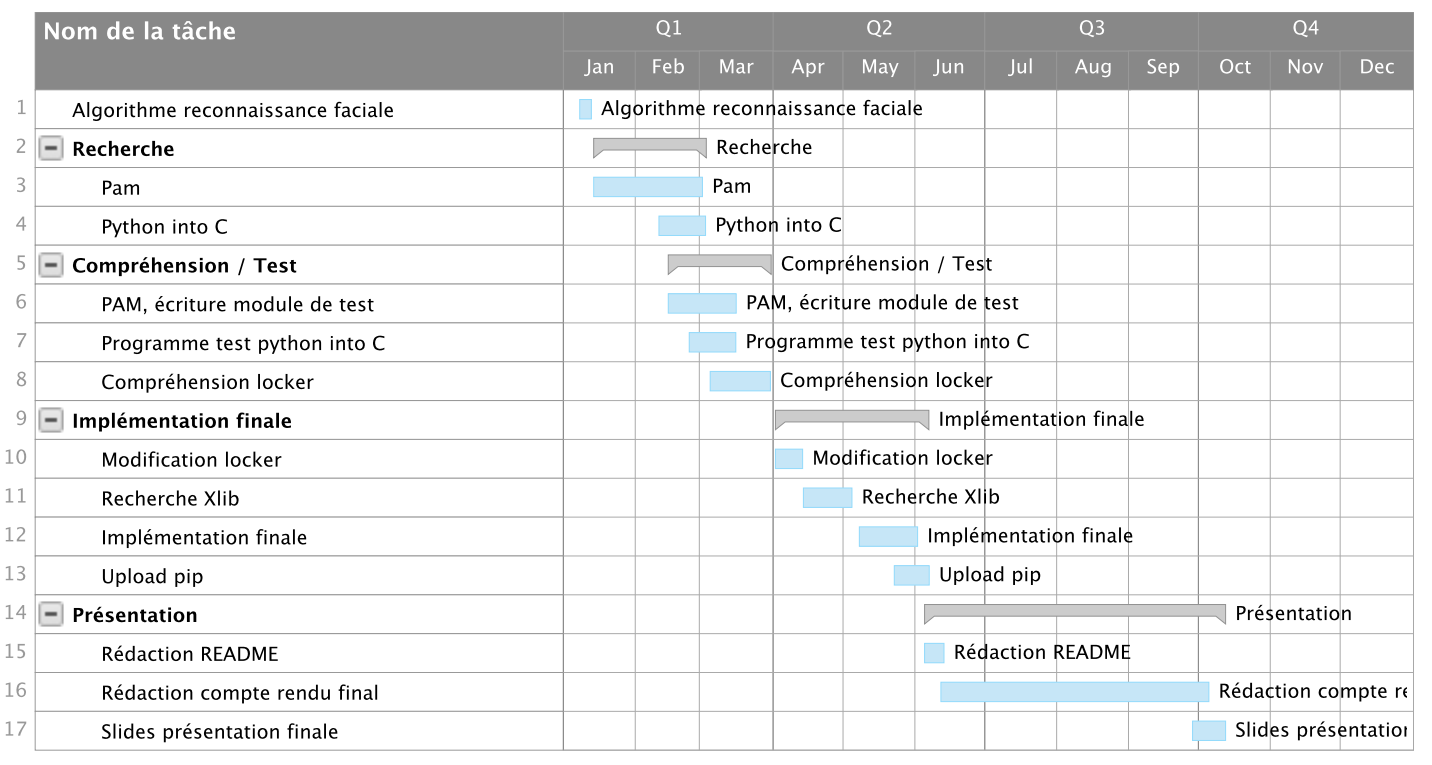
\includegraphics[width=\linewidth]{gantt2}
  \caption{Diagramme de Gantt}
  \label{fig:gantt2}
\end{figure}


\chapter{Technologies utilisées}

\newpage

\section{Liste des technologies explorées}

\begin{itemize}[label=\textbullet, font=\normalfont \color{blue}]
  \item{PAM: Pluggable Authentication Modules}
  \begin{itemize}[label=\textbullet]
    \item{Compréhension globale}
    \item{Config files}
    \item{Ecriture module}
    \item{Implémentation lors du développement}
    \item{Module pam authentication}
  \end{itemize}
  \item{C}
  \begin{itemize}[label=\textbullet]
    \item{Python.c}
    \item{Ecriture locker et module}
  \end{itemize}
  \item{Python}
  \begin{itemize}[label=\textbullet]
    \item{Algorithme reconnaissance faciale}
    \item{Bindings Xlib}
  \end{itemize}
  \item{Xlib}
\end{itemize}

\section{Technologie utilisée – point technique}

\subsection{Xlib - présentation}

Xlib est le nom d'une bibliothèque logicielle, offrant une implémentation de la
partie cliente du protocole \emph{X Window System} en C. Elle contient des fonctions
de bas niveau pour interagir avec un serveur \emph{X}. Ces fonctions permettent aux
programmeurs d'écrire des programmes sans connaître les détails du protocole \emph{X}.
Peu d'applications utilisent la Xlib directement ; en général, elles exploitent
d'autres bibliothèques qui reposent sur la Xlib pour fournir des éléments
d'une interface graphique.\\
Cette bibliothèque est apparue autour de 1985.\\\\
Les versions les plus récentes de plusieurs distributions majeures de Linux utilisent
aujourd'hui \emph{Wayland} plutôt que \emph{X}. Mais \emph{X} détient toujours de loin la plus
grande part d'utilisation. De plus, les programmes codés pour \emph{X} fonctionne
sur \emph{Wayland} grâce au programme de compatibilité \emph{XWayland}. Le contraire n'est pas
possible.

\subsection{Utilisation dans le projet}

Lockatme est un "X locker". C'est-à-dire qu'il fonctionne au niveau du serveur graphique,
dans ce cas la, \emph{X}.

C'est pourquoi nous avons décidé d'utiliser l'API de \emph{X} pour notre projet. C'est par
cette API que l'on peut "grab" le clavier et la souris, c'est-à-dire prendre leur contrôle
et ainsi empêcher leur utilisation en dehors des fonctions souhaitées (délocker le
locker par mot de passe par exemple).

\emph{X} possède en réalité deux API. \emph{Xlib} est très utilisée et plutôt
simple dans son design.
C'est elle que nous avons utilisés. L'API plus récente, \emph{XCB}, présente un
avantage conséquent de performance sur des grosses applications, de par son design
plus complexe, mais à notre échelle, cela importait peu. De plus l'API est encore
très partiellement documenté.

La difficulté se trouve dans le fait que contrairement à une bibliothéque/framework
graphique haut niveau, communiquer avec le serveur graphique directement est
beaucoup plus complexe et fait intervenir des concepts singuliers, pas toujours
simple à saisir. (Voir code en \emph{Annexe: lock.py})

\subsection{Difficultées rencontrée - parallel programming}
Nous souhaitions avoir un locker modulable, qui peut être délocké de plusieurs
façons différentes selon le choix de l'utilisateur (e.g. facial recognition
+ fingerprint reader). Pour cela il nous a fallu choisir une méthode de programmation
parallèle. Les trois choix à disposition pour Python sont le multi-processing,
le multi-threading et les coroutines.

Nous aurions pu utiliser le multi-processing tout comme le multi-threading mais avons donc
opté pour le multi-threading (processus légers) pour utiliser moins de ressources.\\
Quant aux coroutines, nous avons décidé de ne pas utiliser ce processus car l'implémentation
était bien plus compliquée.
\\
Après de nombreux tests sur l'approche à utiliser. Nous avons fini par aboutir sur ce code:

  \begin{minted}{python}
      def add_event(func, event, args_dict):
          def f():
              func(**args_dict)
              event.set()

          return f


      def auth_loop():
          authenticated = Event()
          auth_functions = get_modules_auth_functions()

          for auth_function, options in auth_functions:
              authenticate = add_event(auth_function, authenticated, options)
              t = Thread(target=authenticate)
              t.start()

          authenticated.wait()
    \end{minted}

On crée un objet \emph{threading.Event} dans le programme principal. Tous les modules
utilisés ont accès à l'objet et peuvent "setter" le flag interne à celui-ci de façon
à prévenir le proramme principal si l'utilisateur s'est authentifié avec succès.
Le programme principal attend tout simplement que le flag soit set puis se termine.

\chapter{Version finale}

\newpage

\section{Présentation}
Nous voici donc avec notre application finale écrite en Python, grâce aux bindings
pour Xlib. Elle possède une partie des features que nous souhaitions
implémenter. En effet l'application permet de verrouiller puis de déverrouiller son ordinateur sous linux
en utilisant la reconnaissance faciale grâce à une webcam et une photo placée
en amont dans un dossier spécifique (\emph{cf. 4.3}). L'utilisateur peut également déverrouiller
son écran avec un mot de passe indépendamment de la reconnaissance faciale. C'est
à dire qu'il y a une utilisation de multithread (\emph{cf. 3.2.3}).
L'innovation qui a émergé durant la phase de développement réside dans
l'aspect modulable de l'application, en laissant la possibilité aux utilisateurs
de fork le projet pour créer de nouveaux modules, permettant de proposer de nouvelles manières pour
déverrouiller la machine.\\
L'application possède tout de même quelques points faibles en ce qui concerne la
sécurité et la rapidité de la reconnaissance, assez lente à cause des webcams
d'ordinateur, souvent moins performante.

\section{Structure du projet}
Lockatme se découpe en plusieurs fichier. Le fichier \texttt{\_\_main\_\_.py} est un fichier
spécial en Python, il est le point d'entrée de notre programme. Le fichier \textbf{cli.py}
définit le comportement de la commande "lockatme", c'est-à-dire, les différents
arguments et options disponibles.
Le fichier \textbf{lock.py} contient la fonction de locking qui fait appel à Xlib (\emph{cf. Annexe}).
Le fichier \textbf{auth.py} s'occupe de lire le fichier de configuration de l'utilisateur
puis de lancer les différents threads, chacun faisant appel à la fonction
d'authentification d'un module. Ces fonctions sont définies dans les
fichiers portant le même nom, dans le dossier unlockers (e.g. unlockers/password.py).

\begin{figure}[h]\label{fig:tree}
\begin{center}
  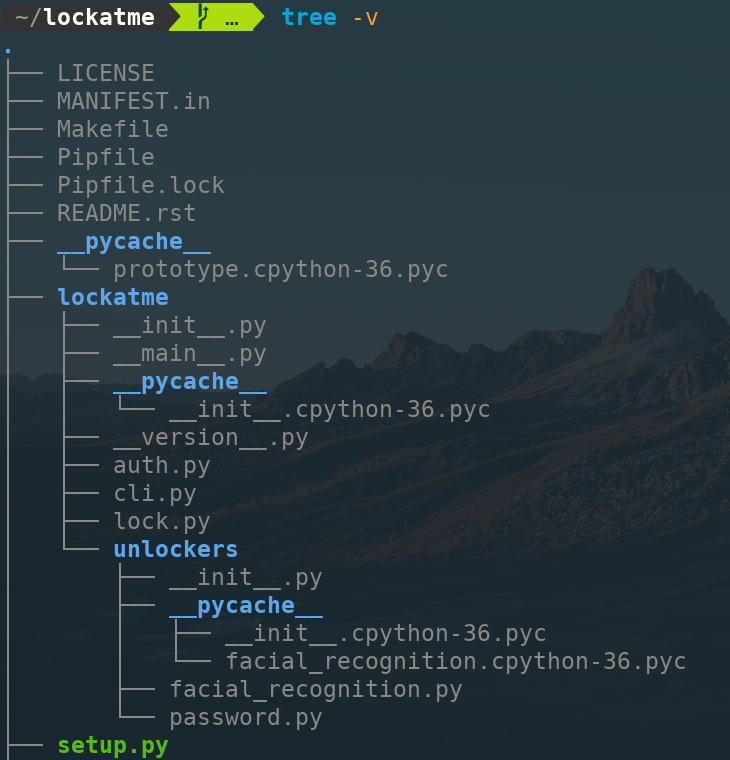
\includegraphics[width=80mm,scale=0.5]{tree}
\end{center}
  \caption{Arborescence du projet}
  \label{fig:tree}
\end{figure}

\section{Utilisation - mode d'emploi}
Le détail de l'utilisation de lockatme est présent sur le repository GitHub :\\
https://github.com/lockatme/lockatme.\\\\
Il suffisait d'une simple commande définit dans le setup.py pour upload sur PyPI (setup.py upload \emph{cf Annexe}).
L'installation peut donc se faire directement grâce à \texttt{pip} :
\begin{lstlisting}[language=bash]
  $ pip install lockatme
\end{lstlisting}

Ensuite dans le fichier configuration, qui se trouve dans \verb|~/.config/lockatme/config|
il est possible de choisir son moyen de déverrouillage sous la section \textbf{[unlockers]}.
\\
L'utilisateur pourra définir directement dans le fichier le \emph{path} vers la photo qui servira
de modèle, dans le cas de la reconnaissance faciale (sous la spécification du module). Le mot de passe, lui, sera celui de
la session active.

\begin{figure}[h]\label{fig:readme}
  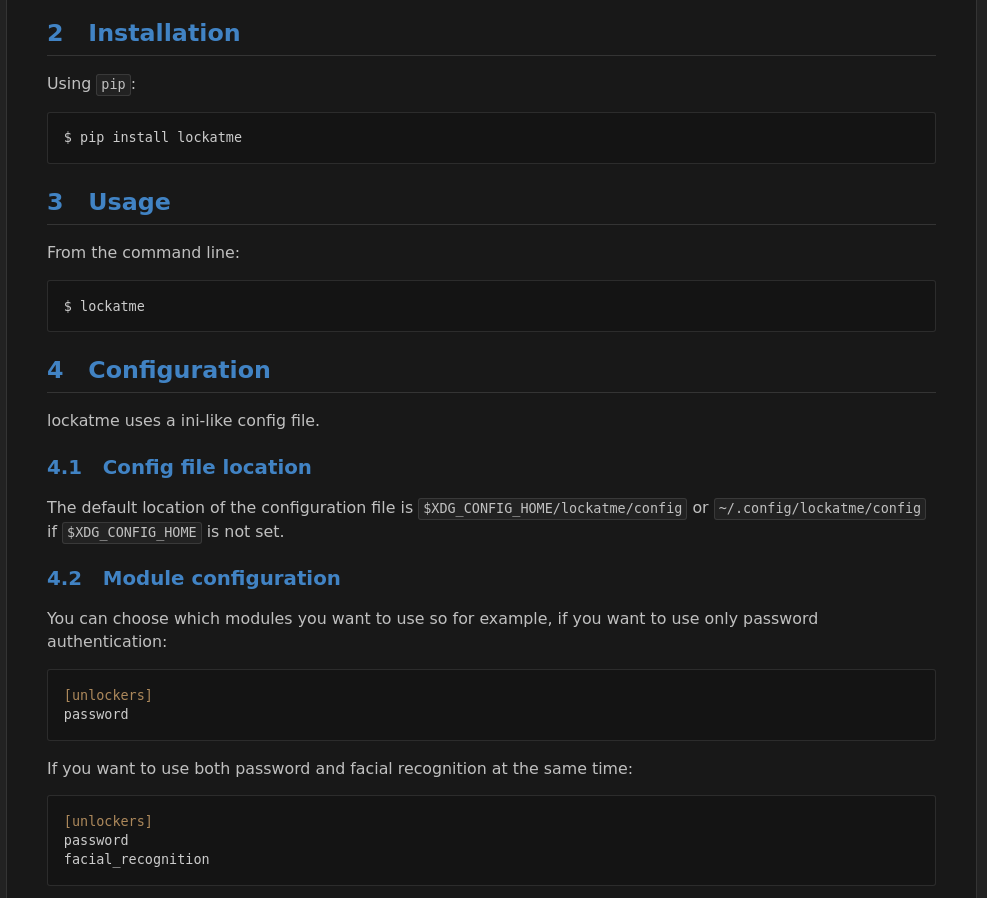
\includegraphics[width=\linewidth]{readme}
  \caption{Extrait README du GitHub}
  \label{fig:readme}
\end{figure}


\chapter{Amélioration possible - conclusion}

\newpage

\section{Interface graphique}
Une des grosses features qui n'est pas présente à la fin du projet est l'interface
graphique. Cependant, pour nous cette aspect n'était pas essentiel étant donné le public ciblé.
En effet ce locker s'adresse surtout à des utilisateurs "geek" qui sont habitués à
l'utilisation de la CLI sur Linux. Nous avons donc consacré tout notre temps à
la fiabilité, à la sécurité du logiciel, et à l'élégance du code.\\\\
Cependant, il serait intéressant tout de même de rendre le logiciel customisable.
Dans un premier temps en ajoutant la possibilité de choisir une image de verrouillage.
Et ensuite d'ajouter une interface graphique qui gère tout de A à Z: choix des options
de verrouillage, choix de la photo modèle (prise en direct avec la webcam via un \emph{face trainer}), choix de
l'image de verrouillage, thèmes, etc...\\
Cependant l'implémentation d'une telle interface (surtout pour la partie \emph{face trainer})
semble être pour le moment en dehors de notre portée.

\begin{figure}[h]\label{fig:facetrain}
  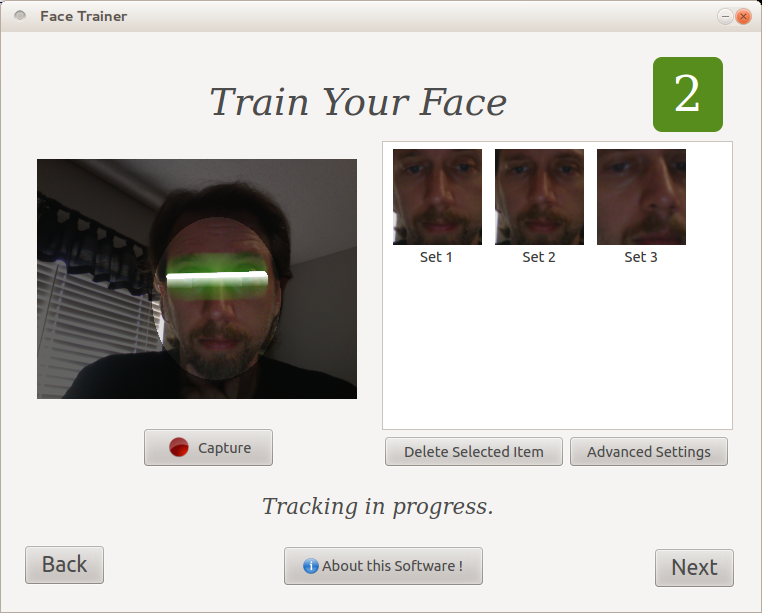
\includegraphics[width=\linewidth]{facetrain}
  \caption{Exemple utilisation d'un face trainer}
  \label{fig:facetrain}
\end{figure}

\newpage

\section{Le futur de lockatme - conclusion}
Le projet lockatme a donc possiblement un futur devant lui, peut être que certains
membres du groupe reviendront sur le projet pour l'améliorer et le rendre pleinement
utilisable au quotidien. De plus le code est open-source et modulable, il est
donc possible qu'une tierse personne fork le projet pour continuer à le faire vivre.\\

Concernant le groupe si nous devions conclure sur la partie technique:\\
Le projet a été très compliqué a cerner, la plus grande partie du travail consistait
à faire des recherches sur des sujets inconnus. Nous pouvons donc dire que le projet
nous a appris énormément de choses sur l'OS Linux (très bas niveaux), sur Python et sur le C
dans une moindre mesure.
\\\\
Sur la partie management et compétences liées au développement:\\
Le projet a été d'autant plus bénéfique sur cet aspect. Chacuns a pu appréhender
la rédaction d'un cahier des charges, la méthodologie Scrum et la communication
au sein d'une équipe pour un projet à long terme. L'apprentissage des compétences liées
au développement, est aussi présent, telle que la maîtrise avancée de Git et GitHub, à travers notamment
l'intégration continue (rédaction de tests) et le travail sur diverses branches aboutissant à des pulls
requests. Il a donc fallu apprendre à travailler en équipe avec ces outils mais aussi
il a fallu apprendre à communiquer avec d'autres outils: Taiga et Discord.
Le projet nous a également montré comment réagir face à l'inconnu total et nous
a aider à améliorer nos capacités de recherches.
\\\\
On peut donc dire que, malgré l'aspect très technique du projet, et la compléxité
de sa mise en place, en lien avec les difficultés de management, chacuns a pu apprendre.
Cette expérience a été sans aucun doute bénéfique pour tous les membres du groupe.




\chapter*{Annexe}

\begin{figure}[h]\label{fig:Taiga}
  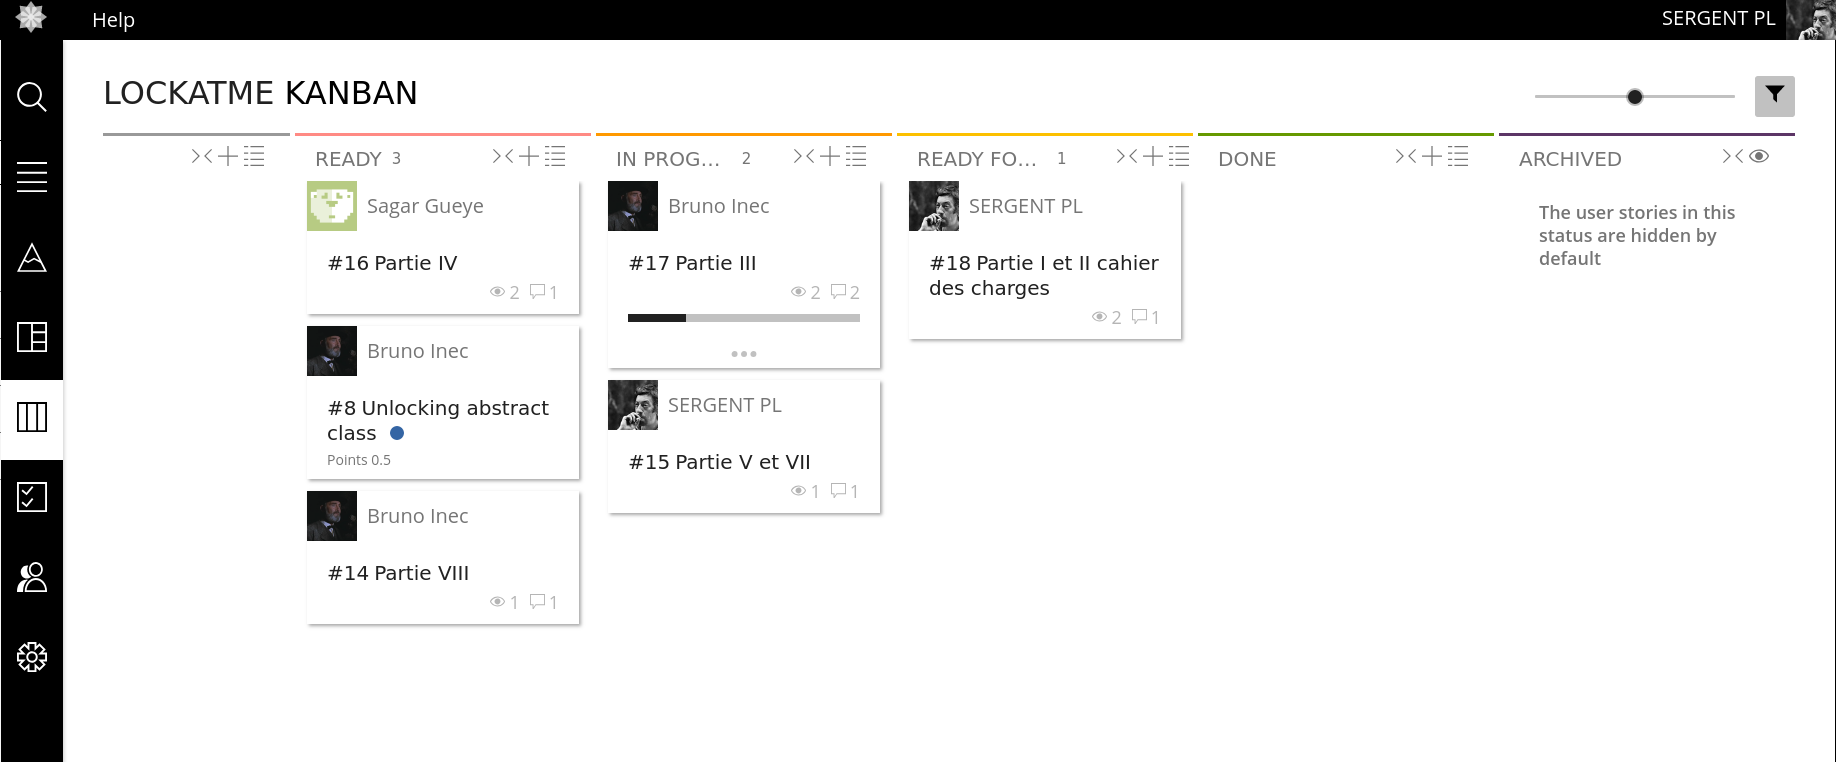
\includegraphics[width=\linewidth]{taiga2}
  \caption{Exemple utilisation taiga}
  \label{fig:Taiga}
\end{figure}

\begin{figure}[h]\label{fig:Taiga}
  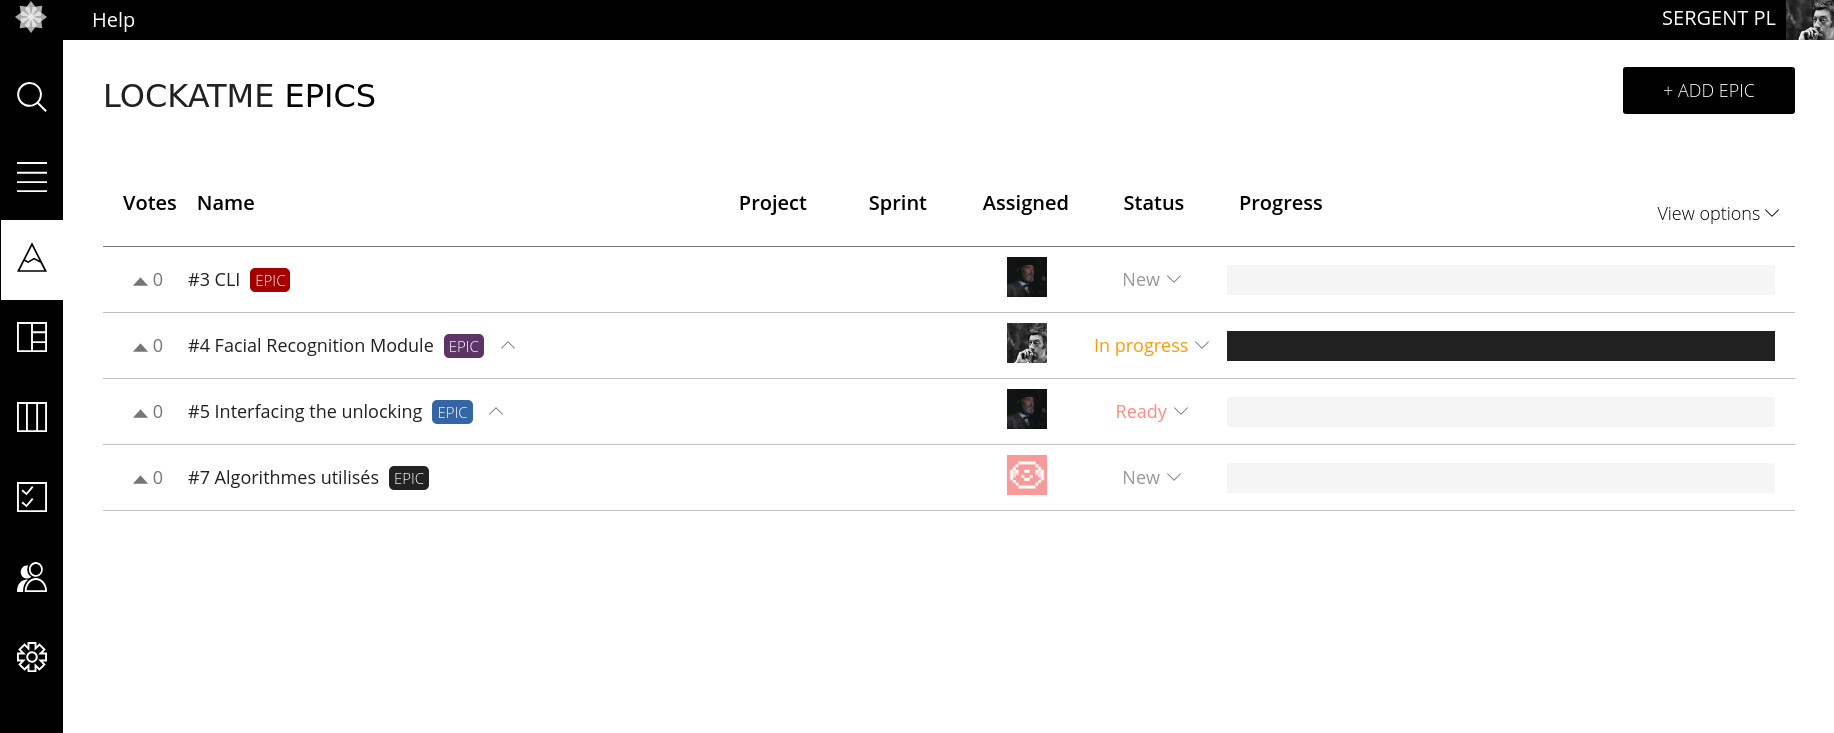
\includegraphics[width=\linewidth]{taiga}
  \caption{Exemple utilisation taiga}
  \label{fig:Taiga}
\end{figure}

\newpage

\begin{minted}{python}
#=====facial_recognition.py=====
  import face_recognition as face
  import cv2


  def is_recognized(model_image_path, test_image):
      model_image = face.load_image_file(model_image_path)

      model_face_encoding = face.face_encodings(model_image)[0]
      test_face_locations = face.face_locations(test_image)
      test_face_encodings = face.face_encodings(test_image, test_face_locations)

      known_faces = [
          model_face_encoding
      ]

      matches = []
      for _, face_encoding in zip(test_face_locations, test_face_encodings):
          matches.append(face.compare_faces(known_faces, face_encoding, tolerance=0.6))

      return any(matches)


  def authenticate(path):
      camera = cv2.VideoCapture(0)

      while True:
          _, shot = camera.read()
          shot = shot[:, :, ::-1]  # Conversion from BGR to RGB
          if is_recognized(path, shot):
              camera.release()
              cv2.destroyAllWindows()
              return
\end{minted}

\newpage

\begin{minted}{python}
#=====lock.py=====#
from Xlib import X, display


def lock_screen(display: display.Display, screen_nb: int):
  screen = display.screen(screen_nb)
  root = screen.root
  display_width = screen.width_in_pixels
  display_height = screen.height_in_pixels

  window = root.create_window(0, 0, display_width, display_height,
                              0, screen.root_depth, window_class=X.CopyFromParent,
                              visual=screen.root_visual,
                              override_redirect=1, background_pixel=screen.black_pixel)

  pixmap = window.create_pixmap(8, 8, 1)
  invisible_cursor = pixmap.create_cursor(pixmap, (0, 0, 0), (0, 0, 0), 0, 0)
  window.change_attributes(cursor=invisible_cursor) # what XDefineCursor does under the hood

  pointer_mask = X.ButtonPressMask | X.ButtonReleaseMask | X.PointerMotionMask
  window.grab_pointer(False, event_mask=pointer_mask,
                      pointer_mode=X.GrabModeAsync, keyboard_mode=X.GrabModeAsync,
                      confine_to=X.NONE, cursor=invisible_cursor, time=X.CurrentTime)

  window.grab_keyboard(True, pointer_mode=X.GrabModeAsync,
                       keyboard_mode=X.GrabModeAsync, time=X.CurrentTime)
  window.map()


def lock(display: display.Display):
  for screen in range(display.screen_count()):
      lock_screen(display, screen)
  display.sync()

\end{minted}
\newpage
\begin{minted}{python}
#=====setup.py=====
#!/usr/bin/env python
import os
import sys
from shutil import rmtree

from setuptools import find_packages, setup, Command

install_requires = [
  'python-xlib'
]
facial_recognition = ['opencv-python', 'dlib', 'face-recognition']
pam_password = ['pamela']
install_requires += facial_recognition + pam_password

tests_require = [
  'pytest'
]

here = os.path.abspath(os.path.dirname(__file__))

with open(os.path.join(here, 'README.rst')) as f:
  long_description = '\n' + f.read()

about = {}
with open(os.path.join(here, 'lockatme/__version__.py')) as f:
  exec(f.read(), about)


class UploadCommand(Command):
  """Support setup.py upload."""

  description = 'Build and publish the package.'
  user_options = []

  @staticmethod
  def status(s):
      """Prints things in bold."""
      print('\033[1m{0}\033[0m'.format(s))

  def initialize_options(self):
      pass

  def finalize_options(self):
      pass

  def run(self):
      try:
          self.status('Removing previous builds…')
          rmtree(os.path.join(here, 'dist'))
      except OSError:
          pass

      self.status('Building Source and Wheel (universal) distribution…')
      os.system('{0} setup.py sdist bdist_wheel --universal'.format(sys.executable))

      self.status('Uploading the package to PyPi via Twine…')
      os.system('twine upload dist/*')

      self.status('Pushing git tags…')
      os.system('git tag v{0}'.format(about['__version__']))
      os.system('git push --tags')

      sys.exit()


setup(
  name='lockatme',
  version=about['__version__'],
  description='Modulable screen locker',
  long_description=long_description,
  author=('Pierre-Louis Sergent, David Anandanadaradja, '
         'Matthieu Kirschleger, Sagar Gueye, Bruno Inec'),
  author_email='brunoinec@gmail.com',
  url='https://github.com/Sweenu/lockatme',
  packages=find_packages(exclude=['tests']),
  entry_points={'console_scripts': ['lockatme = lockatme.__main__:main']},
  python_requires='>=3.6.0',
  install_requires=install_requires,
  tests_require=tests_require,
  include_package_data=True,
  license='MIT',
  classifiers=[
      'Development Status :: 2 - Pre-Alpha',
      'License :: OSI Approved :: MIT License',
      'Intended Audience :: End Users/Desktop',
      'Topic :: Desktop Environment :: Screen Savers',
      'Programming Language :: Python',
      'Programming Language :: Python :: 3',
      'Programming Language :: Python :: 3.6',
      'Programming Language :: Python :: Implementation :: CPython',
      'Operating System :: POSIX :: Linux',
      'Environment :: X11 Applications',
  ],
  cmdclass={'upload': UploadCommand},
)

\end{minted}

\end{document}
